\documentclass{standalone}
\usepackage{tikz}

\begin{document}
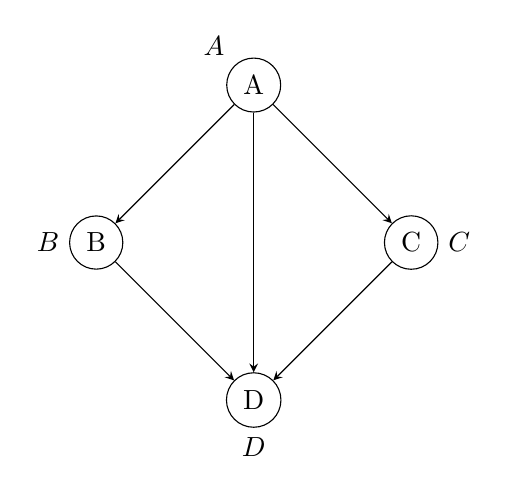
\begin{tikzpicture}[scale=1]
    \node[circle, draw] (A) at (0,0) {A};
    \node[circle, draw] (B) at (-2,-2) {B};
    \node[circle, draw] (C) at (2,-2) {C};
    \node[circle, draw] (D) at (0,-4) {D};

    \draw[-stealth] (A) -- (B);
    \draw[-stealth] (A) -- (C);
    \draw[-stealth] (A) -- (D);
    \draw[-stealth] (B) -- (D);
    \draw[-stealth] (C) -- (D);

    \node[left] at (B.west) {$B$};
    \node[right] at (C.east) {$C$};
    \node[below] at (D.south) {$D$};
    \node[above left] at (A.north west) {$A$};
\end{tikzpicture}
\end{document}